% PLANTILLA APA7
% Creado por: [Tu Nombre]
% Última actualización: [Fecha]
% @COPYLEFT

% Fuentes consultadas (todos los derechos reservados):  
% Normas APA. (2019). Guía Normas APA. [URL de la guía]
% Tecnológico de Costa Rica [Richmond]. (2020, 16 abril). LaTeX desde cero con Overleaf (1 de 3) [Vídeo]. YouTube. [URL del video]
% Weiss, D. (2021). Formatting documents in APA style (7th Edition) with the apa7 LATEX class. [URL del documento]
% @COPYLEFT

% Fuentes consultadas (todos los derechos reservados):  
% Normas APA. (2019). Guía Normas APA. https://normas-apa.org/wp-content/uploads/Guia-Normas-APA-7ma-edicion.pdf
% Tecnológico de Costa Rica [Richmond]. (2020, 16 abril). LaTeX desde cero con Overleaf (1 de 3) [Vídeo]. YouTube. https://www.youtube.com/watch?v=kM1KvHVuaTY Weiss, D. (2021). 
% Formatting documents in APA style (7th Edition) with the apa7 LATEX class. https://ctan.math.washington.edu/tex-archive/macros/latex/contrib/apa7/apa7.pdf @COPYLEFT

%+-+-+-+-++-+-+-+-+-+-+-+-+-++-+-+-+-+-+-+-+-+-+-+-+-+-+-+-+-+-++-+-+-+-+-+-+-+-+-+

% Preámbulo
\documentclass[stu, 12pt, letterpaper, donotrepeattitle, floatsintext, natbib]{apa7}
\usepackage[utf8]{inputenc}
\usepackage{comment}
\usepackage{marvosym}
\usepackage[margin=lin]{geometry}
\usepackage{graphicx}
\usepackage{float}
\usepackage[normalem]{ulem}
\usepackage[spanish]{babel} 
\selectlanguage{spanish}
\useunder{\uline}{\ul}{}
\newcommand{\myparagraph}[1]{\paragraph{#1}\mbox{}\\}
\renewcommand{\headrulewidth}{0pt}
\fancyhead[L]{
        
\includegraphics[width=3.5cm]{usil.png}
}
% Portada
\thispagestyle{empty}
\title{\Large Generación procedural de mapas en videojuegos}
\author{ Salazar Arias, Luis Santiago de Blass \\Bravo Ocampo, David Aquiles \\Flores Grados, Andrea Hilda \\ Narvaez Garriazo, Cristel Margarita
}
% Manera oficial de colocar los autores:
%\author{Autor(a) I, Autor(a) II, Autor(a) III, Autor(a) X}
\affiliation{\Huge\textbf{Universidad San Ignacio de Loyola}}
\course{\normalsize{FC-PREISF03Z01M(H): TEORÍA DE COMPUTACIÓN}}
\professor{ROBERTO JOSUE RODRIGUEZ URQUIAGA}
\duedate{2023}
\begin{document}
\maketitle




% Índices
\pagenumbering{roman}
    % Contenido
\renewcommand\contentsname{\largeÍndice}
\tableofcontents
\setcounter{tocdepth}{2}
\newpage
    % Fíguras
\renewcommand{\listfigurename}{\largeÍndice de fíguras}
\listoffigures
\newpage
    % Tablas
\renewcommand{\listtablename}{\largeÍndice de tablas}
\listoftables
\newpage

% Cuerpo
\pagenumbering{arabic}
\section{\large Agradecimiento}
Queremos expresar nuestro más sincero agradecimiento a todas las personas que nos han brindado su apoyo durante el desarrollo de este proyecto. En primer lugar, deseamos agradecer a nuestro querido profesor, quien generosamente compartió sus conocimientos y nos enseñó a lo largo de todo el ciclo de desarrollo. Su guía y apoyo han sido fundamentales para el éxito de este proyecto.
También queremos extender nuestro agradecimiento a nuestros amigos y familiares, quienes nos han brindado su aliento constante y comprensión en cada etapa de este proceso. Su apoyo incondicional nos ha permitido dedicar las horas necesarias y superar los desafíos que se presentaron en el camino.
Por último, pero no menos importante, queremos expresar nuestro agradecimiento a todos los miembros de la comunidad de programación en línea. Sus valiosas contribuciones en los diferentes foros han enriquecido nuestro aprendizaje y nos han proporcionado una visión más amplia del mundo de la programación.
\newpage
\section{\large Introduccion}
Los videojuegos son una forma de entretenimiento que combina elementos visuales, de audio e 
interactivos para crear experiencias lúdicas y narrativas. Para lograrlo, los desarrolladores de 
videojuegos deben diseñar y programar los escenarios, personajes, objetos y eventos que 
conforman el mundo virtual del juego. Sin embargo, este proceso puede resultar muy costoso y 
requerir mucha mano de obra, especialmente cuando se crea algo grande, variado y detallado. 
Una solución alternativa a este problema es la generación de etiquetas procedimentales, que 
implica el uso de algoritmos y reglas matemáticas para generar contenido de forma automática 
o semiautomática sin la necesidad de un diseño manual. Esta técnica permite crear mapas más 
grandes, más dinámicos y personalizados, ahorrando tiempo y recursos. Algunos ejemplos de 
videojuegos que utilizan generación de mapas procedimentales son Minecraft, No Man's Sky y 
Diablo. Sin embargo, la generación de mapas de procedimientos también implica ciertos desafíos 
y limitaciones, como la coherencia, la unicidad y la jugabilidad del contenido generado. Además, 
se debe considerar la detección de colisiones, que es el proceso de determinar si dos o más 
objetos del juego están en contacto o se superponen. La detección de colisiones es esencial para 
la jugabilidad y la física del juego, ya que te permite simular el comportamiento realista de los 
objetos, así como las interacciones entre ellos y con el jugador. La detección de colisiones puede 
ser muy compleja y exigente desde el punto de vista computacional, especialmente cuando se 
trata de objetos en movimiento o con formas irregulares. Por este motivo, se han desarrollado 
muchas técnicas y algoritmos diferentes para optimizar y simplificar este proceso, como cajas de 
colisión, árboles BSP o propagación de rayos. Estas técnicas varían según el tipo y tamaño del 
objeto, el nivel de precisión requerido y el rendimiento de la máquina. Este trabajo de investigación 
tiene como objetivo analizar las principales técnicas de generación de mapas procedimentales y detección 
de colisiones en videojuegos, así como sus ventajas, desventajas y aplicaciones. Para ello se realizará 
una revisión bibliográfica de las fuentes más relevantes sobre el tema, se explicarán conceptos teóricos 
y se presentarán ejemplos prácticos.\\
\section{\large Marco Teorico}
La generación procedural de mapas se puede definir como el uso de algoritmos para crear contenido para videojuegos sin intervención humana directa. Esta técnica se basa en la definición de reglas, parámetros y funciones que determinan las características del mapa generado, como su forma, tamaño, estructura, color o textura. Estas reglas pueden ser deterministas o aleatorias, lo que implica que el mapa generado sea siempre el mismo o diferente cada vez que se ejecuta el algoritmo. Existen diferentes tipos y niveles de generación procedural de mapas según el grado de control que tenga el desarrollador o el jugador sobre el contenido generado. Se pueden distinguir cuatro niveles: generación offline, generación online, generación interactiva y generación mixta.

En este caso estamos utilizando técnicas y algoritmos para crear contenido de forma automática o semiautomática sin la necesidad de un diseño manual. En particular, estamos utilizando la técnica de generación offline, donde el mapa se genera antes de que el juego empiece y no cambia durante la partida.

Para generar los mapas, estamos utilizando diferentes técnicas y algoritmos. Combinando estas técnicas con otro algoritmo de pathfinding para buscar el "mejor mapa posible". Para mejorar la coherencia y la unicidad del contenido generado, estamos definiendo reglas y parámetros claros y coherentes que determinan las características del mapa generado. También estamos considerando la detección de colisiones, que es esencial para la jugabilidad y la física del juego, y utilizando diferentes técnicas y algoritmos para optimizar y simplificar este proceso. En resumen, nuestro trabajo se enfoca en la generación procedural de mapas en videojuegos utilizando diferentes técnicas y algoritmos para crear contenido de forma automática o semiautomática, y mejorando la coherencia y la unicidad del contenido generado.
\section{\large Metodología}
En el desarrollo de este proyecto, se utilizó una metodología que incluyó diferentes etapas, desde el diseño del estudio hasta el análisis de datos. A continuación, se detalla cada una de estas etapas:

Diseño del estudio:
En esta etapa, se indagó información en papers y artículos para la generación de mapas. Entre las diferentes opciones consideradas, se decidió utilizar el algoritmo de "drunkard's walk" debido a su facilidad de uso. Además, se agregó una variante del algoritmo de búsqueda en amplitud ("breadth first search") para buscar el mapa más "óptimo". Para la lógica del juego en general, se tomaron como referencia algunos video tutoriales, utilizando la librería de Python llamada pygame para crear el juego.

Recopilación de datos:
En esta etapa, se investigaron los papers relacionados con la generación de mapas procedurales. Se tomó la decisión de enfocarse en la generación de mapas en 2D, ya que era más seguro de programar en el nivel y tiempo disponibles. Durante la recopilación de datos, se realizaron resúmenes y lecturas rápidas para seleccionar el código del algoritmo de "drunkard's walk" y el algoritmo de búsqueda en amplitud ("breadth first search"), ya que eran aplicables al proyecto. Por otro lado, se decidió descartar el uso del algoritmo de "perlin noise" debido a que no se ajustaba a las necesidades del proyecto.

Análisis de datos:
En esta etapa, se desarrollaron bocetos e ideas para la creación de un videojuego en 2D. Esto llevó a analizar los papers y video tutoriales que se enfocaban en el desarrollo de juegos RPG de vista superior ("top down"). Gracias a este análisis, se logró construir e implementar el código necesario para la generación de mapas y caminos en el juego.
\noindent \maskCitet{koesnaedi2022}
%\noindent \maskCitet{vilanova2021}\\

\vspace{10pt}
\vspace{10pt}
\vspace{10pt}
\vspace{10pt}
\vspace{10pt}
\vspace{10pt}
\newpage
\section{\large Objetivos}
\subsection{Objetivo general} 
Analizar las principales técnicas de generación de mapas procedimentales y detección de colisiones en videojuegos, así como sus ventajas, desventajas y aplicaciones. Para ello, se realizará una revisión bibliográfica de las fuentes más relevantes sobre el tema, se explicarán conceptos teóricos y se presentarán ejemplos prácticos.
\subsection{Objetivos específicos} 
Explicar la técnica de generación de mapas procedimentales y cómo se utiliza para crear mapas más grandes, dinámicos y personalizados en videojuegos.
Describir la detección de colisiones y su importancia para la jugabilidad y la física del juego.
Identificar los desafíos y limitaciones de la detección de colisiones, especialmente cuando se trata de objetos en movimiento o con formas irregulares.
Presentar diferentes técnicas y algoritmos utilizados para optimizar y simplificar la detección de colisiones, como cajas de colisión, árboles BSP o propagación de rayos.
Analizar las ventajas, desventajas y aplicaciones de las técnicas de generación de mapas procedimentales y detección de colisiones en videojuegos.
\subsection{Diseño de estudio:}
En esta fase, se investigó y buscó información en documentos y artículos para la generación de mapas. Se utilizaron el algoritmo "drunkard's walk" y el algoritmo breadth first search.
Se eligieron estos algoritmos por su funcionalidad y aplicabilidad en el contexto de los videojuegos 2D. Junto con estos algoritmos, se utilizó la librería pygame, que proporciona funciones y herramientas que facilitan la interacción con el desarrollo de juegos 2D, como la reproducción de sonido, la detección de eventos de teclado y la manipulación de gráficos.
\subsection{Recopilación de datos:}
En la recopilación de datos, se investigaron papers y artículos referentes a la generación procedural de mapas y la detección de colisiones. Se realizaron bocetos, utilizando técnicas y conceptos involucrados en estos procesos. Durante esta estapa se descartó el uso del algoritmo de "perlin noise" debido a que no se ajustaba a las necesidades del proyecto. En vez de él se utilizaron  los algoritmos de "drunkard's walk" y el algoritmo de búsqueda en amplitud ("breadth first search"), ya que eran aplicables para el desarrollo de juegos 2D.
\subsection{Análisis de datos:}
Después de la recopilación de datos, se procedió a realizar un análisis exhaustivo y una discusión detallada de los hallazgos más relevantes encontrados en los papers seleccionados. Este análisis permitió obtener una comprensión más profunda de los conceptos teóricos y las técnicas más prometedoras para el proyecto. Se examinaron los diferentes enfoques y se evaluaron sus ventajas y limitaciones en relación con los objetivos y requisitos del proyecto.
\subsection{Resultados:}
Como resultado de un arduo trabajo utilizando la implementación de técnicas sobre generación procedural de mapas y detección de colisiones en videojuegos 2D.
Logramos implementar exitosamente el algoritmo "drunkard´s walk", también conocido coloquialmente como "caminata de borrracho". El cual consta en elegir un punto de partida en el mapa y se elige la dirección mediante las flechas del teclado.  
También se implementó el algoritmo de búsqueda en amplitud ("breadth first search") para buscar el mapa más óptimo. Estos algoritmos permitieron crear mapas grandes, dinámicos y personalizados en el juego, ahorrando tiempo y recursos en el proceso de diseño lo que generó más eficiencia. El juego resultante fue capaz de generar mapas de forma automática y ofrecer una experiencia de juego interesante y desafiante para el usuario.
\begin{figure}
    \centering
    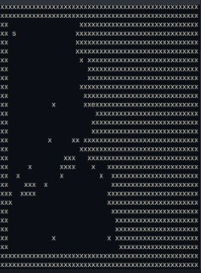
\includegraphics[width=0.5\textwidth]{mapa1.PNG}
    \caption{Primer Mapa Generado}
    \label{fig:enter-label}
\end{figure}
\begin{figure}
    \centering
    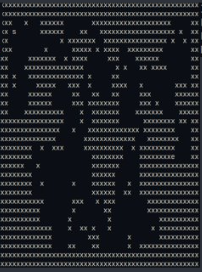
\includegraphics[width=0.5\textwidth]{mapa2.PNG}
    \caption{Segundo Mapa generado}
    \label{fig:enter-label}
\end{figure}
\newpage
\subsection{Conclusiones:}
En conclusión, el diseño de estudio, la recopilación de datos, el análisis de datos y los resultados obtenidos en este proyecto demostraron la viabilidad y efectividad de la generación procedural de mapas y la detección de colisiones en el desarrollo de videojuegos. Estas técnicas ofrecen ventajas significativas en términos de eficiencia y personalización del contenido generado, lo que puede mejorar la experiencia del jugador y optimizar el proceso de desarrollo del juego.
\noindent \maskCitet{smith2021}
%\subsubsection{Título III}
%El resto della concluían sayo de velarte, calzas de velludo para las fiestas, con sus pantuflos de lo mesmo, y los días de entresemana se honraba con su vellorí de lo más fino.
%\paragraph{Título IV}
%Tenía en su casa una ama que pasaba de los cuarenta, y una sobrina que no llegaba a los veinte, y un mozo de campo y plaza, que así ensillaba el rocín como tomaba la podadera.
%\myparagraph{Título IV ii}
%Frisaba la edad de nuestro hidalgo con los cincuenta años; era de complexión recia, seco de carnes, enjuto de rostro, gran madrugador y amigo de la caza. 
%\subparagraph{Título V}
%Quieren decir que tenía el sobrenombre de Quijada, o Quesada, que en esto hay alguna diferencia en los autores que deste caso escriben; aunque por conjeturas verosímiles se deja entender que se llamaba Quijana.

\newpage
% Referencias
\renewcommand\refname{\large\textbf{Referencias}}
\bibliography{mibibliografia}
\end{document}